\documentclass[11pt]{beamer}
\usetheme{Warsaw}
\usepackage[utf8]{inputenc}
\usepackage[french]{babel}
\usepackage[T1]{fontenc}
\usepackage{amsmath}
\usepackage{amsfonts}
\usepackage{amssymb}
\usepackage{graphicx}

\addtobeamertemplate{footline}{\insertframenumber/\inserttotalframenumber}

\author{Arnaud De Bruecker, MediVisu}
\title{MediVisu}

\setbeamercovered{transparent}
\logo{
\includegraphics[width=0.5cm]{esi.png}}
\institute{HEB - ESI} 
\date{juin 2015}

\begin{document}

\begin{frame}
\titlepage
\end{frame}

\begin{frame}
\frametitle{Plan de la présentation}
\tableofcontents
\end{frame}

\section{Contexte}

\begin{frame}
\frametitle{Contexte}
\begin{itemize}[<+->]
\item[•] De multiples fabricants aux solutions propriétaires~;
\begin{itemize}[<+->]
\item[•] Non compatibles entre elles~;
\item[•] Très onéreuses~;
\item[•] Non adaptées à tous les médecins ni aux patients.
\end{itemize}
\item[•] Des alternatives libres existent mais \cdots{}
\begin{itemize}[<+->]
\item[•] Souvent exclusives à une plateforme~;
\item[•] Non certifiées (FDA)~;
\item[•] Pas agréables et simples.
\end{itemize}
\end{itemize}
\end{frame}

\section{Inspiration}

\subsection{Orthanc}

\begin{frame}
\frametitle{Orthanc}

\includegraphics[scale=0.15]{Orthanc.png}
\begin{itemize}[<+->]
\item[•] Projet belge
\item[•] Créé par Sébastien Jodogne
\item[•] Lauréat du prix du logiciel libre en 2014
\item[•] Serveur DICOM pour l'imagerie médicale
\item[•] Licence GPL
\end{itemize}
\end{frame}

\subsection{3DSlicer}

\begin{frame}
\frametitle{3DSlicer}
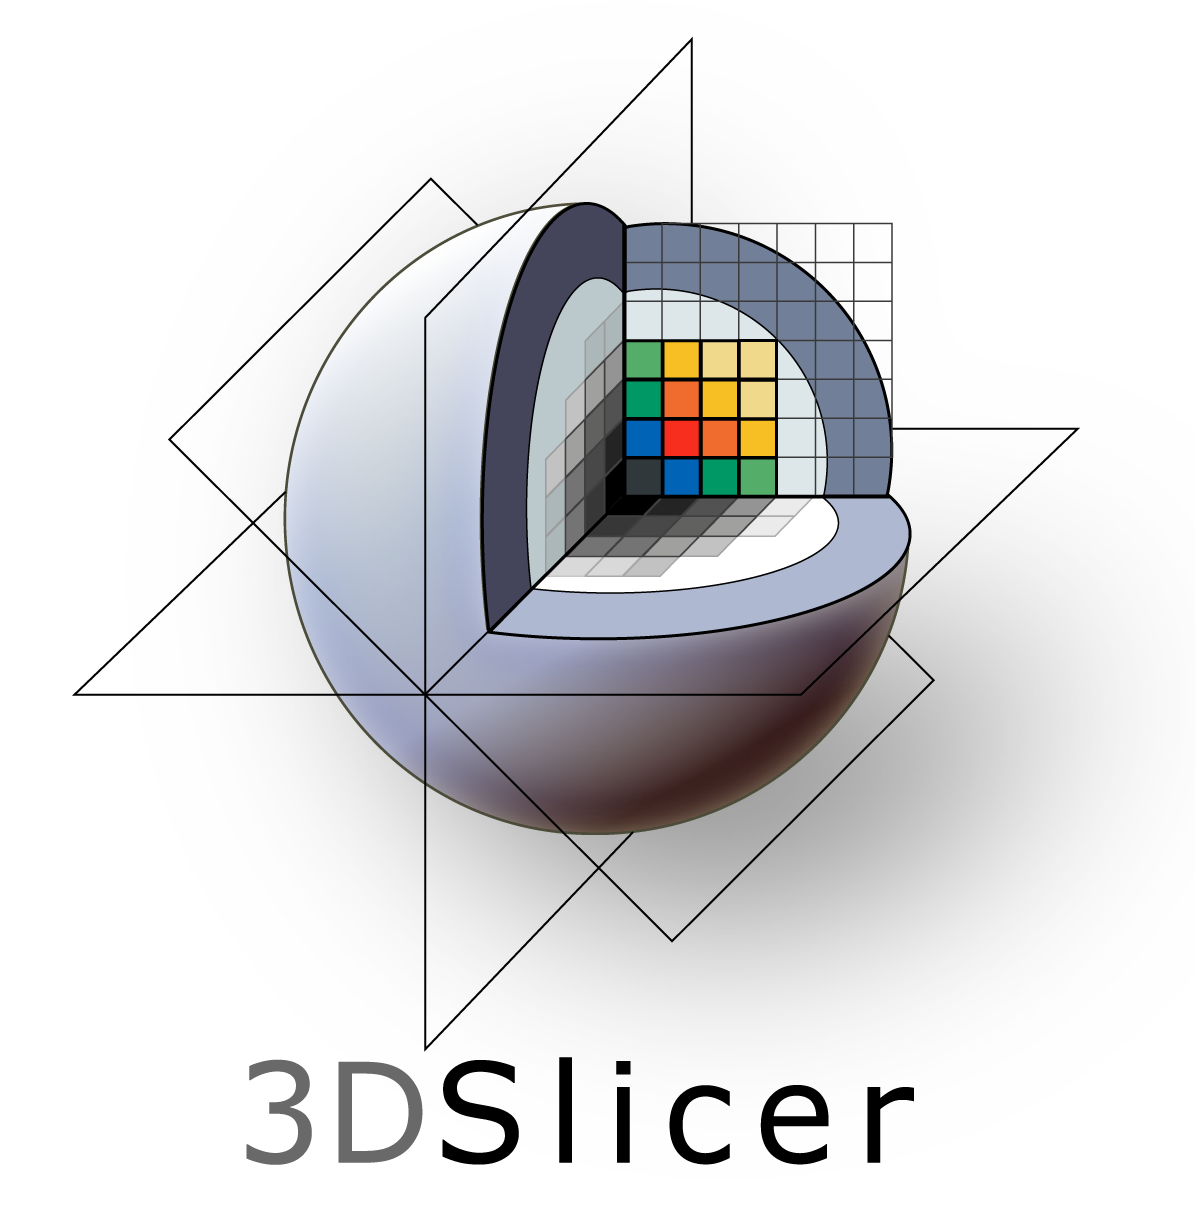
\includegraphics[scale=0.06]{Slicer.png}
\begin{itemize}[<+->]
\item[•] Projet libre mature (17 ans de développement)
\item[•] Grande communauté de développeurs
\item[•] Analyse et manipulation d'images médicales, notamment pour la chirurgie, orienté recherche
\item[•] Licence BSD

\end{itemize}
\end{frame}

\subsection{Osirix}

\begin{frame}
\frametitle{Osirix}

\includegraphics[scale=0.17]{Osirix.jpg}
\begin{itemize}[<+->]
\item[•] Créé par un médecin, Antoine Rosset
\item[•] Très apprécié des professionnels
\item[•] Limité à Mac OS X
\item[•] Licence GPL
\end{itemize}
\end{frame}

\section{Qu'est-ce que le logiciel libre?}

\subsection{Caractéristiques du logiciel libre}

\begin{frame}
\frametitle{Les 4 libertés du logiciel libre}
Modèle de développement participatif basé sur les principes de~:
\begin{itemize}[<+->]
\item[•] liberté d'exécuter le programme par tous ses utilisateurs~;
\item[•] liberté d'étudier le fonctionnement du programme et de l'adapter à ses besoins~;
\item[•] liberté de redistribuer des copies du programme (donner ou vendre)~;
\item[•] liberté d'améliorer le programme et de distribuer ces améliorations au public pour en faire profiter la communauté.
\end{itemize}
\end{frame}

\subsection{Avantages}

\begin{frame}
\frametitle{Avantages}
\begin{itemize}[<+->]
\item[•] Projet ouvert
\begin{itemize}
\item[•] Force de travail exponentielle avec partage des ressources et compétences
\item[•] Maintenance potentiellement assurée
\end{itemize}
\item [] Malheureusement, manque souvent de support utilisateur professionnel facile à identifier
\end{itemize}
\end{frame}

\section{Libre mais pas gratuit}

\subsection{Ambitions commerciales}

\begin{frame}
\frametitle{Ambitions commerciales}
\begin{itemize}[<+->]
\item[•] Support et services aux utilisateurs
\begin{itemize}[<+->]
\item[•] Payant en fonction des priorités
\end{itemize}
\item[•] Formations
\item[•] Certification
\end{itemize}
\end{frame}

\section{Ambitions du logiciel}

\begin{frame}
\frametitle{MediVisu}
MediVisu se veut :
\begin{itemize}[<+->]
\item[•] Libre et le restera : une fondation gèrera les droits
\item[•] Léger et facile à appréhender ("user-friendly")
\item[•] Gestion de profils prédéfinis et modifiables notamment pour chaque spécialisation
\item[•] Multiplateforme (Windows, Mac OS X, GnuLinux au minimum)
\item[•] Certifié pour le diagnostic médical (FDA et équivalent européen)
\item[•] Attention portée sur l'utilisateur
\item[•] Licence AGPL
\end{itemize}
\end{frame}

\begin{frame}
  \frametitle{Liens}
    
  \begin{thebibliography}{10}
        
  \beamertemplatearticlebibitems
 
  \bibitem{3DSlicer}
  	3DSlicer
    \newblock Steve Pieper
    \newblock Disponible sur {\tt http://www.slicer.org}

   \beamertemplatearticlebibitems
 
  \bibitem{Osirix}
  	Osirix
    \newblock Antoine Rosset
    \newblock Disponible sur {\tt http://www.osirix-viewer.com}
    
      \beamertemplatearticlebibitems
 
  \bibitem{Orthanc}
  	Orthanc
    \newblock Sébastien Jodogne
    \newblock Disponible sur {\tt http://www.orthanc-server.com}
 
  \end{thebibliography}
\end{frame}

\end{document}
